\documentclass[12pt, a4paper]{article}
	\input{preambulo}
	 
        
\usepackage{vmargin}
	\setpapersize{A4}
\setmargins{2.5cm}       % margen izquierdo
{1.5cm}                        % margen superior
{16.5cm}                      % anchura del texto
{23.42cm}                    % altura del texto
{10pt}                           % altura de los encabezados
{1cm}                           % espacio entre el texto y los encabezados
{0pt}                             % altura del pie de página
{2cm}                           % espacio entre el texto y el pie de página        




\theoremstyle{definition}
\newtheorem{definition}{Definición}

\theoremstyle{plain}
\newtheorem{lemma}{Lema}

\theoremstyle{plain}
\newtheorem{theorem}{Teorema}

\theoremstyle{plain}
\newtheorem{prop}{Proposición}
        
\begin{document}

 %\title{Lógica Matemática}
%\author{Apuntes del alumno: Javier López}
%\date{2020}
\begin{titlepage}
\centering
\vspace{1cm}
{\bfseries\LARGE Universidad Complutense de Madrid \par}
\vspace{1cm}
{\scshape\Large Facultad de Ciencias Matemáticas \par}
\vspace{2cm}
{\scshape\Huge Lógica Matemática \par}
\vspace{1cm}
{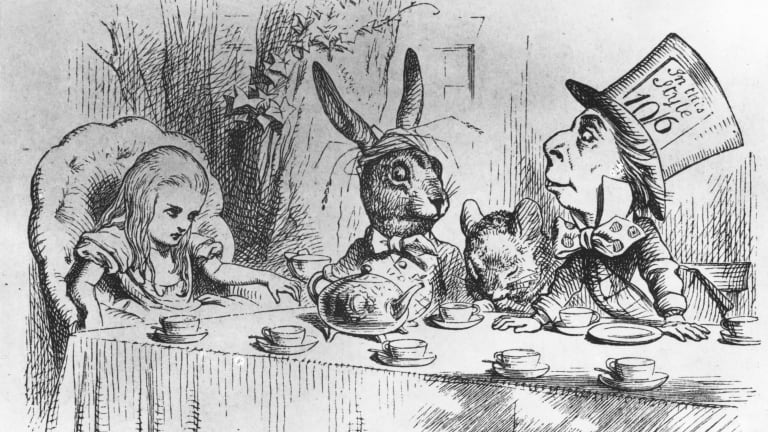
\includegraphics[width=0.7\textwidth]{alice.jpg}\par}
\vspace{3cm}
{\itshape\Large Curso académico 2019-2020 \par}
\vfill
{\Large Autor: Javier López \par}
\vfill
{\Large Versión Febrero 2020 \par}
\end{titlepage}
\newpage
\section*{Fe de errores}
\textit{Este texto está sacado íntegramente de los apuntes que he tomado en clase. Por ello, es más que probable, encontrar en él erratas y errores. Todos ellos pueden {\color{red} ser comunicados a través del foro del campus virtual de la asignatura} y serán subsanados lo antes posible o, en su defecto, añadidos a esta lista para que se tengan en cuenta}.
\begin{itemize}
	\item En el \textit{ejemplo III, el apartado $(\Box)$} no lo tengo escrito en mis apuntes y por tanto la solución no es de Luis. 
	\item Recomiendo revisar el \textit{ejemplo V, caso 4}. 
\end{itemize}
\newpage
\newcommand{\p}[0]{\mbox{PROP}_{SP}}
\newcommand{\cb}[0]{\{ \wedge, \, \lor \, \rightarrow, \, \leftrightarrow \}} 
\newcommand{\boox}[0]{\, \Box \,}
\newcommand{\Mod}[0]{\mbox{Mod}}

\newcommand{\cts}[1]{\mbox{Cts}_{#1}}
\newcommand{\fn}[1]{\mbox{Fn}_{#1}}
\newcommand{\pd}[1]{\mbox{Pd}_{#1}}
\newcommand{\var}[0]{\mbox{Var}}
\newcommand{\term}[1]{\mbox{TERM}_{#1}}
\newcommand{\form}[1]{\mbox{FORM}_{#1}}
\newcommand{\si}[1]{\langle \cts{#1},\, \fn{#1}, \, \pd{#1} \rangle}




	\tableofcontents
	\newpage
     \pagestyle{fancy}
        \setlength\headheight{23pt}
        \fancyhf{}
        \lhead{\bfseries Lógica matemática}
        \chead{}
        \rhead{UCM}
        \lfoot{Curso 19/20}
        \cfoot{}
        \rfoot{\thepage}
        \renewcommand{\headrulewidth}{0.1pt}
        \renewcommand{\footrulewidth}{0.1pt}
%LOGICA PROPOSICIONAL------------------------------------------
     %\newcommand{\p}[0]{\mbox{PROP}_{SP}}
%\newcommand{\cb}[0]{\{ \wedge, \, \lor \, \rightarrow, \, \leftrightarrow \}} 
%\newcommand{\boox}[0]{\, \Box \,}

\section*{Lógica de proposiciones}
\begin{definition} Diremos que una \textbf{proposición} es un enunciado que puede ser verdadero o falso. Nunca será una proposición cualquier enunciado que expresa duda o sentimientos. Tampoco lo serán aquellos enunciados que no tengan sentido lógico. 
\end{definition}
\paragraph{}
Un ejemplo de lo que no es proposición sería
\\
p $\equiv$ ``Juan se cae'' 
\\
q $\equiv$ ``Yo me río''
\\
$\varphi \equiv$ Juan se cae y yo me río  
\paragraph{}
\textbf{Conectivas lógicas}. Son los símbolos que utilizamos para formalizar las proposiciones. Estos son 
\[ \lnot \rightsquigarrow \mbox{ negación} \quad \wedge \rightsquigarrow \mbox{ conjunción} \quad 
\lor \rightsquigarrow \mbox{ disyunción} \quad \rightarrow \rightsquigarrow \mbox{ implicación} \quad
 \]  
 \[\leftrightarrow \rightsquigarrow \mbox{ implicación} \quad \bot \rightsquigarrow \mbox{ falso} \quad 
\top \rightsquigarrow \mbox{ cierto} \]

\begin{definition} Se denomina \textbf{formalizar} una proposición, a escribirla mediante conectivas lógicas. 
\end{definition}
\paragraph{}
\newcounter{ej} %creado el contador ejemplo
\addtocounter{ej}{1} % sumo 1
\textbf{Ejemplo \Roman{ej}}: Formalizar las siguientes frases 
\begin{enumerate}
	\item Si llueve se suspende el partido. 
	\item Solo si llueve se suspende el partido.
\end{enumerate}
tomando como proposiciones p $\equiv$ `` Llueve'' y q $\equiv$ ``se suspende el partido''.
\begin{itemize}
	\item[(1)] $ p\rightarrow q$
	\item[(2)] $ q\rightarrow p$
\end{itemize} 
\paragraph{}
\begin{definition} Llamaremos \textbf{formula} a una cadena de símbolos.
\end{definition}

\begin{definition} Denotamos el \textbf{conjunto de} todos los \textbf{símbolos de proposición} como 
	\[ \mbox{SP}=\{p, \, q, \ldots \} \]
	que es un conjunto numerable (no necesariamente finito). 
\end{definition}

\begin{definition} Al conjunto formado por SP y las conectivas lógicas se le denomina \textbf{alfabeto} y lo denotamos como 
	\[ \mbox{A}= \mbox{SP} \cup \{ \lnot, \, \wedge, \, \lor \, \rightarrow, \, \leftrightarrow, \, (, \, ) \} \]
	denotamos por $\mbox{A}^*$ al \textbf{conjunto de cadenas de símbolos} de A
	\[ \mbox{A}^*=\{ \varepsilon, \, a_1, \, a_2, \ldots , a_n : a_n \geq 0,\, a_i \in A,\, 1 \leq j \leq n   \} \]
	donde $\varepsilon$ es la cadena vacía. 
\end{definition}

\addtocounter{ej}{1} % sumo 1
\textbf{Ejemplo \Roman{ej}}: Dado el vocabulario $\mbox{A}=\{ a, \,b \}$ su conjunto de cadena de símbolos será el conjunto 
\[ \mbox{A}^*= \{\varepsilon, \, a, b, ab, ba, aaa, aab, \ldots \} \]
\begin{definition} Dado SP un conjunto de símbolos de proposición, tomamos el alfabeto $\mbox{A}_{SP}$ y definimos $\mbox{PROP}_{SP}$ como el menor subconjunto de $\mbox{A}^*_{SP}$ que verifica 
\begin{enumerate}
	\item $SP \subseteq \mbox{PROP}_{SP}$
	\item Si $\varphi \in \p$, entonces $(\lnot \varphi) \in \p$
	\item Si $\varphi, \psi \in \p$, entonces $(\varphi \, \Box \, \psi) \in \p$, donde \[ \Box \in \cb \] 
\end{enumerate}
\end{definition}
Veamos como se construye esta definición. Sean 
\[ P_0 = \mbox{SP} \]
\[ P_{n+1}= P_n \cup \{(\lnot \varphi), \, (\varphi \, \Box \, \psi) : \, \Box \in \cb, \, \varphi, \psi \in P_n \} \]
\[ P= \bigcup_{i \geq 0} \]
veamos como $P$ cumple las propiedades 1, 2 y 3 de la definición anterior. De forma trivial se verifica que $\p \subseteq P$ y nos faltaría por demostrar la inclusión en el otro sentido. 
\begin{proof}
Sea $\varphi \in P$ entonces $\exists k$ tal que $\varphi \in P_k$ y aplicamos inducción sobre $k$ para ver que $\varphi \in \p$. 
\paragraph{}
Para $k=0$, por la propiedad 1 de la definición se tienen que $\varphi \in \p$. Para $k \geq 0$ 
\begin{itemize}
	\item[(i)] $\varphi \in P_{k-1}$
	\item[(ii)] $\psi \in P_{k-1}$ tal que $\varphi = (\lnot \psi)$
	\item[(iii)] $\psi_1, \psi_2 \in P_{k-1}$ entonces $\varphi = (\psi_1 \boox \psi_2)$
\end{itemize}
\end{proof} %28/01/2020
     \subsection{Inducción estructural}
Supongamos que queremos probar una propiedad $P$ que cumpla $P(\varphi), \forall \varphi \in \p$. Para ello vamos a usar una estructura basada en el \textit{método de inducción} usual sobre $\mathbb{N}$ aplicado sobre las proposiciones. El método tiene la siguiente estructura 
\begin{itemize}
	\item[(1)] Demostrar la \textbf{base inductiva}. Lo haremos sobre las atómicas (\textit{i.e.} SP, $\bot, \top$)
	\begin{itemize}
		\item[(AT)] Se cumple $P(\varphi), \forall \varphi \in \mbox{AT}$.
	\end{itemize}
	\item[(2)] \textbf{Paso inductivo}. Una vez que tenemos la propiedad $P$ probada para el caso base, suponemos la cierta la hipótesis de inducción, es decir que se cumple $P(\varphi),$ y la utilizamos para los dos casos siguientes
	\begin{itemize}
		\item[$(\lnot \varphi)$] Utilizando la \textit{h.i.} demostraremos que se cumple $P((\lnot \varphi))$.
		\item[($\Box$)] Suponemos que $\varphi_1$ cumple $P$ y que $\varphi_2$ cumple $P$, es decir, se verifican $P(\varphi_1)$ y $P(\varphi_2)$ y entonces hay que demostrar $P(\varphi_1 \boox \varphi_2)$ con $\Box \in \cb$. Dependiendo de la propiedad que queramos demostrar, podremos, o bien agrupar la conectivas lógicas en un sólo caso, o bien separarlas de forma en casos particulares. 
	\end{itemize}
\end{itemize} 
\addtocounter{ej}{1} % sumo 1
\textbf{Ejemplo \arabic{ej}}: Vamos a demostrar por inducción estructural la siguiente propiedad
\begin{center}
P: \textit{Toda fórmula tiene el mismo número de paréntesis abiertos y cerrados}
\end{center}
Para ello, vamos a denotar $\vert \varphi \vert_{(}$ al número de paréntesis abiertos de $\varphi$ y, análogamente, denotamos $\vert \varphi \vert_{)}$ al número de paréntesis cerrados de $\varphi$.
\paragraph{}
\begin{itemize}
	\item[(AT)] Si $\varphi \in SP$ ó $\varphi=\bot$ ó $\varphi=\top$, en cualquiera de los casos no hay paréntesis, luego $\vert \varphi \vert_{(}=\vert \varphi \vert_{)}$ y por tanto se verifica
	\[ P(\varphi), \forall \varphi \in \mbox{AT} \]
	\item[$(\lnot \varphi)$] Sea $\varphi \in \p$ tal que se verifica $P(\varphi)$, es decir 
	\[ \vert \varphi \vert_{(}=\vert \varphi \vert_{)} \]
	ahora, el $\vert (\lnot \varphi) \vert_{(}= \vert \varphi \vert_{(} +1$ y analogamente $\vert (\lnot \varphi) \vert_{)}= \vert \varphi \vert_{)} +1$, luego por \textit{h.i.} se tiene que 
	\[ \vert (\lnot \varphi) \vert_{)}=\vert (\lnot \varphi) \vert_{(}  \]  
	luego se verifica $P(\lnot \varphi), \forall \varphi \in \p$.
	\item[($\Box$)] Sean $\varphi_1, \, \varphi_2 \in \p$, supongamos que
	\[ \mbox{Se verifica } P(\varphi_1) \Rightarrow \vert \varphi_1 \vert_{(}=\vert \varphi_1 \vert_{)}  \]
	\[ \mbox{Se verifica } P(\varphi_2) \Rightarrow \vert \varphi_2 \vert_{(}=\vert \varphi_2 \vert_{)}  \]  
	y veamos que ocurre con $P(\varphi_1 \boox \varphi_2)$ 
	\[ \vert \varphi_1 \boox \varphi_2 \vert_{(}= \vert \varphi_1 \vert_{(} + \vert \varphi_2 \vert_{(} +1  \]
	\[ \vert \varphi_1 \boox \varphi_2 \vert_{)}= \vert \varphi_1 \vert_{)} + \vert \varphi_2 \vert_{)} +1  \]
	y, por \textit{h.i.} se tiene que  
	\[ \vert \varphi_1 \boox \varphi_2 \vert_{)}= \vert \varphi_1 \boox \varphi_2 \vert_{(} \]
	finalizando así la demostración.
\end{itemize}

\begin{definition} Sea A un alfabeto y $\omega \in A^*$ decimos que $\omega'$ es \textbf{prefijo} de $\omega$ si $\exists \omega''$ tal que 
\[ \omega=\omega' \omega'' \]
con, $\omega=a_1 \ldots a_n$, entonces $\exists k, \, 0\leq k \leq n$ tal que $\omega'=a_1 \ldots a_k$. Diremos que $\omega'$ es \textbf{prefijo propio} si $\omega' \neq \varepsilon$ y $\omega' \neq \omega$. 
\end{definition}

\addtocounter{ej}{1} % sumo 1
\textbf{Ejemplo \arabic{ej}}: Sea $A=\{ a,\,b \}$ y $\omega=aababb$ entonces 
\begin{multicols}{2}
\begin{itemize}
	\item Si $k=0 \Rightarrow \omega'=\varepsilon$
	\item Si $k=1 \Rightarrow \omega'=a$
	\item Si $k=2 \Rightarrow \omega'=aa$
	\item Si $k=3 \Rightarrow \omega'=aab$
	\item Si $k=4 \Rightarrow \omega'=aaba$
	\item Si $k=5 \Rightarrow \omega'=aabab$
	\item Si $k=5 \Rightarrow \omega'=\omega$		
\end{itemize}
\end{multicols}
\addtocounter{ej}{1} % sumo 1
\textbf{Ejemplo \arabic{ej}}: Sea $\varphi'$ prefijo propio de $\varphi$, vamos a probar por inducción estructural la propiedad 
\begin{center}
P: \textit{El número de paréntesis cerrados de $\varphi'$ es menor que el número de paréntesis abiertos}.
\end{center}
utilizando la notación del ejemplo (III).
\begin{itemize}
	\item[(AT)] Sea $\varphi \in SP$, supongamos $\varphi=p$ entonces, o bien $\varphi'=\epsilon$ o $\varphi'=p$ luego $\varphi$ no tiene prefijos propios de modo que se cumple la propiedad. Si $\varphi=\bot$ o $\varphi = \top$ de nuevo $\varphi'=\epsilon$ o $\varphi'=\bot$ o $\varphi'=\top$ que no son prefijos propios, luego $\varphi$ tampoco tiene prefijos. 
	\[ P(\varphi), \forall \varphi \in \mbox{AT} \]
	\item[($\lnot \varphi$)] Supongamos que $\varphi'$ es prefijo propio de $(\lnot \varphi)$, y supongamos que todo prefijo propio de $\varphi$ cumple la propiedad. 
	\begin{itemize}
		\item[(CASO 1)] Si $\varphi'=($, entonces $\vert \varphi' \vert_{(}=1 > \vert \varphi' \vert_{)}=0$
		\item[(CASO 2)] Si $\varphi'=(\lnot$, entonces $\vert \varphi' \vert_{(}=1 > \vert \varphi' \vert_{)}=0$
		\item[(CASO 3)] Si $\varphi'=(\lnot \varphi''$, siendo $\varphi''$ prefijo de $\varphi$ luego cumple la propiedad, si además le sumamos uno la cumple también. 
		\item[(CASO 4)] Si $\varphi'=(\lnot \varphi$, entonces $\vert \varphi' \vert_{(}=1 = \vert \varphi' \vert_{)}=0 $
\end{itemize}	 
 \item[($\Box$)] Supongamos que todo prefijo propio de $\varphi_1$,  $\varphi_2$ cumple la propiedad. Hay que ver entonces, que los prefijos lo cumplen 
 \[(, \, (\varphi_1, \, \varphi_1, \, \varphi_1 \boox, \, (\varphi_1 \boox \varphi_2', \, (\varphi_1 \boox \varphi_2  \]
 \begin{flushright}
 \textit{Se deja como ejercicio}.
 \end{flushright}
\end{itemize} %29/01/2020
     \subsection*{Definiciones recursivas}
Supongamos que queremos definir una función 
\[ H: \p \rightarrow A \]
donde $A$ puede tomar diferentes tipos de conjunto: $\mathbb{N}$, $\mathcal{P}(\p)$,... para hacerlo de forma recursiva, vamos a necesitar las siguientes funciones auxiliares
\begin{itemize}
	\item Caso atómico
	\[ H_{\mbox{AT}}: \mbox{AT} \rightarrow A \]
dada por $H(\varphi)=H_{\mbox{AT}}(\varphi), \forall \varphi \in \mbox{AT}$
	\item Paso recursivo: donde diferenciamos entre la negación y las conectivas binarias. 
	\begin{itemize}
		\item[(i)] Negación 
		\[ H_{\lnot}: A \rightarrow A \]
		dada por 
	\[ H \vert (\lnot \varphi) \vert = H_{\lnot}\vert (H(\varphi) \vert \]
		\item[(ii)] Conectivas binarias 
		\[ H_{\Box}: A \times A \rightarrow A \]
		dada por 
	\[ H \vert (\varphi_1 \boox \varphi_2) \vert = H_{\Box}\vert (H(\varphi_1, \, \varphi_2) \vert \]
	\end{itemize}
\end{itemize} 
En los casos (i) e (ii) ni la entrada ni la salida de la función está formada por formulas. 
\paragraph{}
\addtocounter{ej}{1} % sumo 1
\textbf{Ejemplo \Roman{ej}}: Si queremos definir de forma recursiva el número de paréntesis abiertos de una proposición
\[ H_{(}: \p \rightarrow \mathbb{N} \] 
se tendría
\[ H_{\mbox{AT}\,(}: \mbox{AT} \rightarrow \mathbb{N} \]
dada por
\[ H_{\mbox{AT}\,(}(\varphi)=0, \forall \varphi \in \mbox{AT} \]
la negación
\[ \begin{matrix}
 H_{\lnot \,(}: & \mathbb{N} & \rightarrow & \mathbb{N}\\
 &n& \longmapsto &  n+1
\end{matrix} \] 
finalmente, el resto de conectivas 
\[ \begin{matrix}
 H_{\Box \,(} :  & \mathbb{N} \times \mathbb{N} & \rightarrow & \mathbb{N}\\
 &(n,\, m)& \longmapsto &  n+m+1
\end{matrix} \] 
Escribirlo así es un poco farragoso por lo que, generalmente, escribiremos las funciones haciendo uso del propio concepto de recursión
\[ H_{(}(\varphi)=0, \forall \varphi \in \mbox{AT} \]
\[ H_{\lnot \,(}((\neg \varphi))=H_{(}(\varphi) +1 \]
\[ H_{\Box \,(}(\varphi_1 \boox \varphi_2)= H_{(}(\varphi_1)+H_{(}(\varphi_2)+1 \]
además, en la escritura, se suprime la función auxiliar. 
\addtocounter{ej}{1} % sumo 1
\textbf{Ejemplo \Roman{ej}}: definiremos de forma recursiva el número de apariciones de $\wedge$ en $\varphi$ y lo denotamos como $\vert \varphi \vert^{\wedge}$.
\begin{itemize}
	\item[(AT)] $\vert \varphi \vert^{\wedge}=0, \forall \varphi \in \mbox{AT}$
	\item[($\neg$)] $\vert (\neg \varphi) \vert^{\wedge}=\vert \varphi \vert^{\wedge}$
	\item[($\Box$)] Hay que diferenciar dos casos
	\[ \vert (\varphi_1 \boox \varphi_2) \vert^{\wedge}= \left\lbrace \begin{matrix}
	\vert \varphi_1 \vert^{\wedge}+\vert \varphi_2 \vert^{\wedge}& \mbox{si}& \Box \in \{ \lor, \, \rightarrow, \, \leftrightarrow\}\\
	\\
	\varphi_1 \vert^{\wedge}+\vert \varphi_2 \vert^{\wedge}+1 & \mbox{si}& \Box=\wedge
\end{matrix} \right.	 \] 
\end{itemize}
\begin{definition} Dadas dos fórmulas $\varphi$ y $\psi$ decimos que $\psi$ es una \textbf{subformula} de $\varphi$ si una parte de $\varphi$ formada por símbolos consecutivos es idéntica a $\psi$.
\end{definition}
\addtocounter{ej}{1} % sumo 1
\textbf{Ejemplo \Roman{ej}}: dada la formula, 
\[ \varphi \equiv (p \lor (q \rightarrow (\neg r))) \]
observamos que esta formada por las subformulas siguientes
\[ p, \, q, \, r \, (\neg r), \, (q \rightarrow (\neg r)), \varphi \]
\addtocounter{ej}{1} % sumo 1
\textbf{Ejemplo \Roman{ej}}: Creamos una función recursiva que devuelva las diferentes subformulas de una formula dada.
\[ \mbox{SUB}: \p \rightarrow \mathcal{P}(\p) \]
dada por 
\begin{itemize}
	\item[(AT)] $\mbox{SUB}(\varphi)=\{\varphi \}, \forall \varphi \in \mbox{AT}$
	\item[($\neg$)] $\mbox{SUB}((\neg \varphi))=\{ (\neg\varphi)\} \cup \mbox{SUB}(\varphi)$
	\item[($\Box$)] $ \mbox{SUB} ((\varphi_1 \boox \varphi_2) )= \mbox{SUB}(\varphi_1)+\mbox{SUB}(\varphi_2) \cup \{ (\varphi_1 \boox \varphi_2) \}$
\end{itemize}
\begin{prop} El esquema de definición recursiva da como resultado una única función. Esto es, dadas 
\[ H_{\mbox{AT}}: \mbox{AT} \rightarrow A \]
\[ H_{\lnot}: A \rightarrow A \]
\[ H_{\Box}: A \times A \rightarrow A \]
existe una única función $H: \p \rightarrow A$ que verifica 
\[ H(\varphi)=H_{\mbox{AT}}(\varphi), \forall \varphi \in \mbox{AT} \]
\[H((\neg \varphi))=H_{\neg}(H (\varphi))\]
\[H ( (\varphi_1 \boox \varphi_2) ) = H_{\Box}(H(\varphi_1, \, \varphi_2))\]
\end{prop}
\subsection*{Eliminación de paréntesis}
Como en la aritmética básica, cuando escribimos una operación podemos utilizar las reglas de prioridad, asociatividad, etc. para escribir el menor número de paréntesis posible. Así por ejemplo en 
\[ (((2 \cdot 3)+5)-(3 \cdot 2))=2 \cdot 3 +5-3\cdot 3 \]
la idea es, por tanto, dar una serie de reglas para poder hacer lo mismo con nuestras formulas de proposición. 
\subsubsection*{Reglas de eliminación de paréntesis}
\begin{enumerate}
	\item \textbf{Elminación de paréntesis externos}. No aportan información.
	\item \textbf{Prioridad entre conectivas}. En la siguiente lista, las conectivas, aparecen de más prioridad a menos
	\[ (+)\quad \neg, \, \wedge, \, \lor, \, \rightarrow, \, \leftrightarrow \quad (-) \]
	\item \textbf{Asociatividad}. Adoptamos el convenio de asociar por la izquierda. De este modo si tenemos $p \rightarrow q \rightarrow r$ daremos como asociación válida 
	\[ (p \rightarrow q) \rightarrow r \]
	siendo, por tanto, errónea 
	\[ p \rightarrow (q \rightarrow r)  \]
	Esto mismo se aplica para $\leftrightarrow$. En los casos de $\vee$ y $\wedge$ no se presenta problema pues son asociativas.
\end{enumerate} %30/01/2020
     \subsection*{Valoraciones: Tablas de verdad}
Todo lenguaje se subdivide en 
\begin{enumerate}
	\item Sintaxis: reglas de formación de las frases o fórmulas. 
	\item Semántica: significado de las frases o fórmulas. 
\end{enumerate}
de este modo, se conforma un lenguaje formal. 

\begin{definition} Denotaremos por $\mbox{BOOL}$ al conjunto formado por dos elementos\footnote{Durante este curso elegimos, generalmente, como notación para el conjunto BOOL $=\{$V, F$\}$.} 
\[ \mbox{BOOL}= \{\mbox{Verdadero}, \mbox{ Falso} \}=\{\mbox{V}, \mbox{ F} \}=\{\mbox{T}, \mbox{ F} \}=\{1,\, 0\} \]
con los que vamos a \textit{valorar} las fórmulas. 
\end{definition}

Para dar un sentido más formal a la idea de \textit{valorar}, vamos a construir una serie de aplicaciones sobre el conjunto BOOL en la siguiente definición. 
\begin{definition} Diremos que una \textbf{valoración} es una aplicación de la forma 
\[ \begin{matrix}
v: & \mbox{SP} & \rightarrow &\mbox{BOOL}\\
\end{matrix} \]
cuya extensión da lugar a 
\[ \begin{matrix}
\widehat{v}: & \p & \rightarrow &\mbox{BOOL}\\
&\varphi &  \mapsto & \widehat{v}(\varphi)
\end{matrix} \]
que definiremos de forma recursiva
\begin{itemize}
	\item[(AT)] $\widehat{v}(\top)=V$, $\widehat{v}(\bot)=F$, $\widehat{v}(p)=v(p), \mbox{ si } p \in \mbox{SP}$
	\item[($\neg$)] $\widehat{v}(\neg)=v_{\neg}(\widehat{v}(\varphi))$
	\item[($\Box$)] $\widehat{v}((\varphi \boox \psi))= v_{\Box}(\widehat{v}(\varphi), \, \widehat{v}(\psi))$ con $\Box \in \cb$
\end{itemize}
\end{definition}

Estas funciones de valoración dan lugar a las tablas de verdad de cada una de las conectivas lógicas. 
\paragraph{}
Las aplicaciones son
\[ \begin{matrix}
v_{\Box}: & \mbox{BOOL}\times \mbox{BOOL} & \rightarrow &\mbox{BOOL}\\
\end{matrix} \]
si $\Box \in \cb$
En el caso de la negación
\[ \begin{matrix}
v_{\neg}: & \mbox{BOOL} & \rightarrow &\mbox{BOOL}\\
\end{matrix} \]
\begin{table}[]
\centering
\begin{tabular}{ccccc|ccccc|ccccc|ccccc|ccc}
\multicolumn{4}{c}{$p \wedge q$}                                                                      &  & \multicolumn{4}{c}{$p \lor q$}                                                                      &  & \multicolumn{4}{c}{$p \rightarrow q$}                                                                     &  & \multicolumn{4}{c}{$p \leftrightarrow q$}                                                                     &  & \multicolumn{3}{c}{$\neg p$}                                                 \\ \hline
                                        &                                   & p          &            &  &                                         &                                 & p          &            &  &                                         &                                        & p          &            &  &                                         &                                            & p          &            &  &                                         &                                 &   \\ \cline{3-4} \cline{8-9} \cline{13-14} \cline{18-19}
                                        & \multicolumn{1}{c|}{$v_{\wedge}$} & \textbf{V} & \textbf{F} &  &                                         & \multicolumn{1}{c|}{$v_{\lor}$} & \textbf{V} & \textbf{F} &  &                                         & \multicolumn{1}{c|}{$v_{\rightarrow}$} & \textbf{V} & \textbf{F} &  &                                         & \multicolumn{1}{c|}{$v_{\leftrightarrow}$} & \textbf{V} & \textbf{F} &  &                                         & \multicolumn{1}{c|}{$v_{\neg}$} &   \\ \cline{2-4} \cline{7-9} \cline{12-14} \cline{17-19} \cline{22-23} 
\multicolumn{1}{c|}{\multirow{2}{*}{q}} & \multicolumn{1}{c|}{\textbf{V}}   & V          & F          &  & \multicolumn{1}{c|}{\multirow{2}{*}{q}} & \multicolumn{1}{c|}{\textbf{V}} & V          & V          &  & \multicolumn{1}{c|}{\multirow{2}{*}{q}} & \multicolumn{1}{c|}{\textbf{V}}        & V          & F          &  & \multicolumn{1}{c|}{\multirow{2}{*}{q}} & \multicolumn{1}{c|}{\textbf{V}}            & V          & F          &  & \multicolumn{1}{c|}{\multirow{2}{*}{p}} & \multicolumn{1}{c|}{\textbf{V}} & F \\
\multicolumn{1}{c|}{}                   & \multicolumn{1}{c|}{\textbf{F}}   & F          & F          &  & \multicolumn{1}{c|}{}                   & \multicolumn{1}{c|}{\textbf{F}} & V          & F          &  & \multicolumn{1}{c|}{}                   & \multicolumn{1}{c|}{\textbf{F}}        & V          & V          &  & \multicolumn{1}{c|}{}                   & \multicolumn{1}{c|}{\textbf{F}}            & V          & V          &  & \multicolumn{1}{c|}{}                   & \multicolumn{1}{c|}{\textbf{F}} & V
\end{tabular}
\end{table}

Donde encontremos matrices simétricas, podemos decir que ese operador es conmutativo. Los operadores que conmutan son: la disyunción y la conjunción.
\paragraph{}
\addtocounter{ej}{1} % sumo 1
\textbf{Ejemplo \Roman{ej}}: utilizando las aplicaciones de la definición (10), vamos a valor la fórmula 
\[ \varphi= (q \lor r) \rightarrow (q \rightarrow r) \]
partiendo de las valoraciones 
\[v(p)=V, \quad v(q)=F, \quad v(r)=V \]
\[ \widehat{v}= v_{\rightarrow}(\widehat{v}(q \lor r), \widehat{v}(p \rightarrow q)) =  v_{\rightarrow}(v_{\lor}(\widehat{v}(q), \widehat{v}(r)), v_{\rightarrow}(\widehat{v}(p), \widehat{v}(q))= \]
\[ =v_{\rightarrow}(v_{\lor}(F,V), v_{\rightarrow}(V,F))= v_{\rightarrow}(V,F)=F \]

Es claro que no es un método muy óptimo si queremos ver todas las posibles valoraciones de las proposiciones que formen parte de la fórmula. Para ello se utiliza la tabla de verdad. 
\paragraph{}
\addtocounter{ej}{1} % sumo 1
\textbf{Ejemplo \Roman{ej}}: Completar la tabla de verdad de la fórmula $\varphi$ del ejemplo anterior. (\textit{Se deja como ejercicio)}.

\begin{definition} Dada $v: \mbox{SP} \rightarrow \mbox{BOOL}$ valoración y $\varphi \in \p$, $v$ \textbf{satisface} $\varphi$ si y sólo si $\widehat{v}(\varphi)=V$; y denotamos $v \models \varphi$. En caso contrario, $v$ no satisface $\varphi$, si $\widehat{v}(\varphi)=F$, denotamos $v \not\models \varphi$. Al símbolo $\models$ se le denomina \textbf{símbolo de satisficidad}.
\end{definition}

\subsubsection*{Clasificación de fórmulas}
\begin{definition} Según como sean las valoraciones de una fórmula, podemos clarificarlas en
\begin{enumerate}
	\item \textbf{Satisfactible}. Existe alguna valoración $v$ tal que $v \models \varphi$.
	\item \textbf{Tautología}. Siempre es cierto, es decir, $\forall v$ se tiene que $v \models \varphi$.
	\item \textbf{Contingencia}. $\varphi$ se dice contingencia si es satisfactible, pero no tautología. 
	\item \textbf{Contradicción}. Siempre es falso, es decir, $\forall v$ se tiene que $v \not \models \varphi$.
\end{enumerate}
\end{definition}
\paragraph{}
\newcounter{obs} %creado el contador ejemplo
\addtocounter{obs}{1} % sumo 1
\textbf{Observación}. Todas las valoraciones posibles que hay en una fórmula viene dado por $2^{\rho}$ donde $\rho$ es el número de proposiciones que tiene la fórmula. %3/02/2020
     %\addtocounter{ej}{1} % sumo 1
%\textbf{Ejemplo \arabic{ej}}:
\begin{definition} Sea $\Phi \subseteq \p$ un conjuntos de fórmulas, definimos 
\[ \Mod (\Phi)= \{ v / v \models \varphi, \forall \varphi \in \Phi \} \]
entonces diremos que 
\begin{enumerate}
	\item $\Phi$ es \textbf{satisfactible}, si $\Mod (\Phi) \neq \emptyset$ y denotamos $\mbox{Sat}(\Phi)$
	\item $\Phi$ es \textbf{insatisfactible}, si $\Mod (\Phi) = \emptyset$ y denotamos $\mbox{Insat}(\Phi)$
	\item $\varphi \in \p$ es \textbf{consecuencia lógica} de $\Phi$ si y sólo si $\Mod (\Phi) \subseteq\Mod (\{\varphi \})$, denotamos $\Phi \models \varphi$.
\end{enumerate} 
\end{definition}
\paragraph{}
\addtocounter{obs}{1}
\textbf{Observación}: si partimos de una premisa falsa podemos concluir cualquier cosa. Esto es 
\[ \mbox{Insat}(\Phi) \mbox{ entonce } \Phi \models \varphi \]
además, podemos expresar una tautología como 
\[ \mbox{Si } \Phi \neq \emptyset \mbox{ y } \Phi \models \varphi \mbox{ entonce } \models \varphi \]
En este sentido se pueden definir todo tipo de propiedades, como las que vienen a continuación. 

\begin{prop} Se tiene que 
\begin{enumerate}
	\item $\Phi \cup \{ \varphi \} \models \psi$ si y sólo si $\Phi \models \varphi \rightarrow \psi$
	\item $\Phi \models \varphi$ si y sólo si $\textrm{Insat}(\Phi \cup \{\varphi\})$
\end{enumerate}
\end{prop}
\begin{proof}
Vamos a demostrar el apartado (1) (\textit{el (2) queda como ejercicio}. Comenzamos con la implicación hacía la derecha. 

Supongamos que $\Phi \cup \{\varphi\} \models \psi$ y hay que ver si $\Mod (\Phi) \subseteq \Mod (\varphi \rightarrow \psi)$. Si $v \in \Mod (\Phi)$ entonces 
\begin{itemize}
	\item[(i)] $\widehat{v}(\varphi)=V \Rightarrow v \in \Mod(\varphi) \Rightarrow v \in \Mod (\Phi \cup\{\varphi\} \Rightarrow v \in \Mod (\psi) \Rightarrow \widehat{v}(\psi)=V$ de modo que $\widehat{v}(\varphi \rightarrow \psi)=V$ en consecuencia $v \in \Mod (\varphi \rightarrow \psi)$.
	\item[(ii)] $\widehat{v}(\varphi)=F$, entonces $\widehat{v}(\varphi \rightarrow \psi)=V \Rightarrow v \in \Mod (\varphi \rightarrow \psi)$ 
\end{itemize}

Para la implicación en el otro sentido. Si $v \in \Mod(\Phi \cup \{ \varphi \})$ entonces 
\[ \left. \begin{matrix}
v \in \Mod (\Phi) &\Rightarrow & v \in \Mod (\varphi \rightarrow \psi) &\Rightarrow & \widehat{v}(\varphi \rightarrow \psi)=V\\
v \in \Mod (\varphi) &\Rightarrow & \widehat{v}(\varphi)=V
\end{matrix} \right \rbrace \Rightarrow \widehat{v}(\psi)=V \Rightarrow v \in \Mod(\psi) \] 
\end{proof} %4/02/2020
     %Clase completa de problemas 
	 \subsection{Equivalencias lógicas}
Acabamos de ver en la \textit{proposición 2} que podemos escribir propiedades acerca de un conjunto de proposiciones. Pero, de momento, los métodos que disponemos para demostrar este tipo de propiedades no siempre son los más óptimos. Veamoslo en con el siguiente ejemplo.
\paragraph{}
\addtocounter{ej}{1} % sumo 1
\textbf{Ejemplo \Roman{ej}}: a través de una tabla de verdad, partiendo de 
\[ \Phi=\{ \neg p \wedge q \rightarrow r,\, \neg p,\, \neg r \} \]
\[ \varphi= \neg q\]
hay que demostrar que 
\[ \Phi \models \varphi \]
Para la tabla coloreamos en rojo las premisas que deben satisfacer la consecuencia, pintada de azul. Satisfacer implica que la valoración debe ser V en todas las premisas. Esta situación sólo se da para las valoraciones $p, \, q$ y $r$ todas ellas F (fila señalada con una flecha). 

\begin{table}[h]
\centering
\begin{tabular}{lc|c|c|c|c|c|c||c}
\cline{2-9}
                  & \textbf{p} & \textbf{q} & \textbf{r} & {\color[HTML]{FE0000} \textbf{$\neg p$}} & \textbf{$\neg p \wedge q$} & {\color[HTML]{FE0000} \textbf{$\neg p \wedge q \rightarrow r$}} & {\color[HTML]{FE0000} \textbf{$\neg r$}} & {\color[HTML]{3531FF} \textbf{$\neg q$}} \\ \cline{2-9} 
                  & \textbf{V} & \textbf{V} & \textbf{V} & F                                        & F                          & {\color[HTML]{32CB00} V}                                        & F                                        & F                                        \\ \cline{2-9} 
                  & \textbf{V} & \textbf{V} & \textbf{F} & F                                        & F                          & {\color[HTML]{32CB00} V}                                        & {\color[HTML]{32CB00} V}                 & F                                        \\ \cline{2-9} 
                  & \textbf{V} & \textbf{F} & \textbf{V} & F                                        & F                          & {\color[HTML]{32CB00} V}                                        & F                                        & V                                        \\ \cline{2-9} 
                  & \textbf{V} & \textbf{F} & \textbf{F} & F                                        & F                          & {\color[HTML]{32CB00} V}                                        & {\color[HTML]{32CB00} V}                 & V                                        \\ \cline{2-9} 
                  & \textbf{F} & \textbf{V} & \textbf{V} & {\color[HTML]{32CB00} V}                 & V                          & {\color[HTML]{32CB00} V}                                        & F                                        & F                                        \\ \cline{2-9} 
                  & \textbf{F} & \textbf{V} & \textbf{F} & {\color[HTML]{32CB00} V}                 & V                          & F                                                               & {\color[HTML]{32CB00} V}                 & F                                        \\ \cline{2-9} 
                  & \textbf{F} & \textbf{F} & \textbf{V} & {\color[HTML]{32CB00} V}                 & F                          & {\color[HTML]{32CB00} V}                                        & F                                        & V                                        \\ \cline{2-9} 
$\longrightarrow$ & \textbf{F} & \textbf{F} & \textbf{F} & {\color[HTML]{32CB00} V}                 & F                          & {\color[HTML]{32CB00} V}                                        & {\color[HTML]{32CB00} V}                 & V                                        \\ \cline{2-9} 
\end{tabular}
\end{table}

puesto que la consecuencia es también verdadera, hemos demostrado que $\Phi \models \varphi$. 
\paragraph{}
Esta forma no es efectiva y vamos a dar mecanismos para no tener que hacer uso de valoraciones y tablas de verdad. 

\begin{definition} Sean $\varphi, \, \psi \in \p $ son \textbf{lógicamente equivalentes} y lo denotamos como $\varphi \sim \psi$, si y sólo si $\forall v, \widehat{v}(\varphi)=\widehat{v}(\psi)$.
\end{definition}

\begin{lemma}
Diremos que $\sim$ es una \textbf{relación de equivalencia}; más aún, es una congruencia respecto a dos operadores lógicos (\textit{i.e.} la relación se respeta con los operadores lógicos). 
\[ \left. \begin{matrix}
\varphi \sim \psi & \varphi_1 \sim \varphi'_1\\
\neg \varphi \sim \neg \psi & \varphi'_2 \sim \varphi_2 
\end{matrix} \right \rbrace  \Rightarrow \quad \varphi_1 \boox \varphi_2 \sim \varphi'_1 \boox \varphi'_2\]
con $\Box \in \cb$.
\end{lemma}

\subsubsection{Leyes de equivalencia lógica}
\begin{enumerate}
	\item \textbf{Conmutatividad}
	\[ p \wedge q \sim q \wedge p \]
	\[ p \lor q \sim q \lor p \]
	\item \textbf{Asociatividad}
	\[ p \wedge (q \wedge r) \sim (p \wedge q) \wedge r \]
	\[ p \lor (q \lor r) \sim (p \lor q) \lor r \]
	\item \textbf{Idempotencia}
	\[ p \wedge p \sim p\]
	\[ p \lor p \sim p\]
	\item \textbf{Distributiva}
	\[ p \wedge (q \lor r) \sim (p \wedge q) \lor (p \wedge r) \]
	\[ p \lor (q \wedge r) \sim (p \lor q) \wedge (p \lor r) \]
	\item \textbf{Absorción}
	\[ p \wedge (q \lor p) \sim p \]
	\[ p \lor (q \wedge p) \sim p \]
	\item \textbf{Cero y uno}
	\[ p \wedge \top \sim p \]
	\[ p \lor \top \sim \top \]
	
	\[ p \wedge \bot \sim \bot \]
	\[ p \lor \bot \sim p \]
	\item \textbf{Contradicción}
	\[ p \wedge (\neg p) \sim \bot \]
	\item \textbf{Tercio excluido}
	\[ p \lor (\neg p) \sim \top \]
	\item \textbf{Doble negación}
	\[ \neg (\neg p) \sim p \]
	\item \textbf{Reducción}
	\[ p \rightarrow q \sim \neg p \lor q \]
	\[ p \leftrightarrow q \sim (p \rightarrow q) \wedge (q \rightarrow p) \]
	\item \textbf{De Morgan}
	\[ \neg(p \wedge q) \sim \neg p \lor \neg q\]
	\[ \neg(p \lor q) \sim \neg p \wedge \neg q\]
\end{enumerate}

Se deja como ejercicio simplificar las expresiones siguientes mediante las leyes que acabamos de ver 
\begin{enumerate}
	\item $ \{ \varphi_1, \varphi_2 \} \models \psi $
	\item $ \mbox{Insat}(\Phi \cup \{\psi\} ) $
	\item $ \varphi_1 \wedge \varphi_2 \wedge \neg \psi \sim \bot $
\end{enumerate} %6/02/2020
	 \subsection{Sustitución}
La idea es tomar una parte de una formula y sustituirla por algo equivalente que sea más manejable. Definamos de forma rigurosa el concepto. 

\begin{figure}[h]
\centering

\includegraphics[width=8cm]{susti}
\end{figure}

\begin{definition} Sean $\varphi, \, \psi \in \p$ y $p \in \mbox{SP}$, se denota
\[ \psi[\varphi/p] \]
a sustituir en la fórmula $\psi$ las apariciones de $p$ por $\varphi$. Para definir la sustitución utilizamos el método de recursión. De este modo, obtenemos 
\begin{itemize}
    \item[(AT)] Para las formulas atómicas se tiene que
    \begin{itemize}
    	\item $p[\varphi/p] = \varphi$.
    	\item $q[\varphi/p] = q \quad q \neq p$.
    	\item $\top[\varphi/p] = \top$.
    	\item $\bot[\varphi/p] = \bot$.
    \end{itemize}
    \item[($\neg$)] $(\neg\psi)[\varphi/p] = \neg(\psi[\varphi/p])$.
    \item[($\Box$)] $(\psi_1 \boox \psi_2)[\varphi/p] = (\psi_1[\varphi/p] \boox \psi_2[\varphi/p])$.
\end{itemize}
\end{definition}

De manera esquemática 

\begin{figure}[h]
\centering

\includegraphics[width=4cm]{esq}
\end{figure}

\begin{theorem}
Sean $\varphi, \varphi', \psi \in \p$, $p \in SP$. Si $\varphi \sim \varphi'$, entonces $\psi[\varphi/p] \sim \psi[\varphi'/p]$.
\end{theorem}

\textbf{Notación}. Dada
\[f:  A  \rightarrow  B\]
se tiene que
\[f[b/a](x)= \left \lbrace \begin{matrix}
f(x) & \mbox{si} & x \neq a\\
b & \mbox{si} & x = a
\end{matrix}\right. \]

\begin{lemma}
Sean $\varphi, \psi \in \p$, $p \in \mbox{SP}$ y $v$ valoración. Entonces:
\[ \widehat{v}(\psi[\varphi/p]) =  v[\widehat{\widehat{v}(\varphi)/p}](\psi)\]
\end{lemma}
\begin{proof}
Procedemos por inducción estructural sobre $\psi$. Comenzamos por las atómicas
\begin{itemize}
\item[(AT)]
\begin{itemize}
	\item Si $\psi = p$ entonces, $\psi[\varphi/p] = \varphi$. Luego 
    	 \[ \widehat{v}(\psi[\varphi/p]) = \widehat{v}(\varphi) \]
   	\item Si $\psi = q$ con $q \neq p$ entonces $\psi[\varphi/p] = q$, con lo que $\widehat{v}(\psi[\varphi/p]) = \widehat{v}(q)$, luego 
   	\[ v[\widehat{\widehat{v}(\varphi)/p}](q) = \widehat{v}(q) \]
   	\item Si $\psi = \top$, $\psi[\varphi/p] = \top$, luego 
   	\[ v[\widehat{\widehat{v}(\varphi)/p}](\top) = v(\top) = V \]
   	\item Si $\psi = \bot$, $\psi[\varphi/p] = \bot$, luego 
   	\[ v[\widehat{\widehat{v}(\varphi)/p}](\bot) = v(\bot) = F \]
\end{itemize} 
\item[($\neg$)] Si $\psi = \neg \psi_1$, entonces $\widehat{v}((\neg\psi_1)[\varphi/p]) = \widehat{v}(\neg(\psi_1[\varphi/p])) = v_{\neg}(\widehat{v}(\psi_1[\varphi/p]))$ por hipótesis de inducción tenemos que
\[  v_{\neg}(v[\widehat{\widehat{v}(\varphi)/p}])(\psi_1) = v[\widehat{\widehat{v}(\varphi)/p}](\neg\psi_1) \]   
\item[($\Box$)] Si $\psi = \psi_1 \boox \psi_2$, entonces 
\[ \widehat{v}(\psi[\varphi/p]) = \widehat{v}((\psi_1[\varphi/p]  \boox  \psi_2[\varphi/p])) = v_{\Box}(\widehat{v}(\psi_1[\varphi/p]), \; \widehat{v}(\psi_2[\varphi/p])) \]
 por hipótesis de inducción  
 \[ v_{\Box}(v[\widehat{\widehat{v}(\varphi)/p}](\psi_1), \; v[\widehat{\widehat{v}(\varphi)/p}](\psi_2)) = v[\widehat{\widehat{v}(\varphi)/p}](\psi_1 \boox \psi_2) \]
\end{itemize}
\end{proof}

\begin{proof}(\textit{Teorema 1}). 
\[ \widehat{v}(\psi[\varphi/p]) = v[\widehat{\widehat{v}(\varphi)/p}](\psi) =_{1} v[\widehat{\widehat{v}(\varphi')/p}](\psi) = \widehat{v}(\psi[\varphi'/p])\]
en (1) utilizamos que $\widehat{v}(\varphi)=\widehat{v}(\varphi')$.
\end{proof}

\addtocounter{ej}{1} % sumo 1
\textbf{Ejemplo \Roman{ej}}: Sean $\varphi=p \rightarrow q$ y $\psi=r \rightarrow t$ y tomamos la sustitución $\psi[\varphi/r]=(p \rightarrow q) \rightarrow t$. Entonces, es indiferente valorar $\psi[\varphi/r]$ en
 
\begin{center}
\begin{tabular}{|c|c|c|c|}
\hline 
\textbf{p} & \textbf{q} & \textbf{r} & \textbf{t} \\ 
\hline 
V & F & V & V \\ 
\hline 
\end{tabular}
\end{center}
 
que valorarlo, siendo $\widehat{v}(\varphi)=F$, entonces $v[\widehat{v}(\varphi)/r]$

\begin{center}
\begin{tabular}{|c|c|c|c|}
\hline 
\textbf{p} & \textbf{q} & \textbf{r} & \textbf{t} \\ 
\hline 
V & F & F & V \\ 
\hline 
\end{tabular} 
\end{center}
\paragraph{}
\begin{lemma}
Si $\psi_1 \sim \psi_2$ entonces $\psi_1[\varphi/p] \sim \psi_2[\varphi/p]$.
\end{lemma}
\begin{proof}
En efecto
\[ \widehat{v}(\psi_1[\varphi/p]) = v[\widehat{\widehat{v}(\varphi)/p}](\psi_1)=\]
como $\psi_1 \sim \psi_2$
\[  v[\widehat{\widehat{v}(\varphi)/p}](\psi_2)=\widehat{v}(\psi_2[\varphi/p]) \]
\end{proof}

\addtocounter{ej}{1} % sumo 1
\textbf{Ejemplo \Roman{ej}}: Si queremos ver $\varphi \wedge \psi \sim \psi \wedge \varphi$ basta tomar $\psi_1= p \wedge \psi$ y $\psi_2= \psi \wedge p$ y aplicar el lema anterior. 
\paragraph{}
\textbf{Observación}. Esto implica que, gracias al lema de sustitución, las leyes de equivalencia vistas en la sección \ref{sec:Leyes de equivalencia logica}, es también aplicable a fórmulas completas.  %10/02/2020
	 \subsection{Completitud funcional}
Debido a las leyes de reducción los operadores $\rightarrow, \, \leftrightarrow$ se dicen secundarios. También podemos definir nuevos operadores como 
\begin{center}
 $\begin{array}{ccc}
 \mbox{Disyunción exclusiva}  & \veebar & p\veebar q \sim (p \lor \neg q) \lor (\neg p \lor q) \\ 
 \mbox{NAND} & \downarrow & p\downarrow q \sim \neg( p \lor q) \\ 
 \mbox{NOR} & \uparrow & p\uparrow q \sim \neg( p \wedge q)
 \end{array}  $ 
 \end{center} 
 o a través de una tabla de verdad  
\begin{center}
 \begin{tabular}{|c|c|c|c|c|}
 \hline 
 p & q & $p\veebar q$ & $p\downarrow q$ & $p\uparrow q$ \\ 
 \hline 
 V & V & F & F & F \\ 
 \hline 
 V & F & V & V & F \\ 
 \hline 
 F & V & V & V & F \\ 
 \hline 
 F & F & F & V & V \\ 
 \hline 
 \end{tabular} 
\end{center}
\paragraph{}
Podríamos construir un operador lógico con tantos argumentos como deseáramos. Pero, vamos a ver que todos ellos se pueden expresar de forma equivalente como conjunción, negación y disyunción. 
\begin{figure}[h]
\centering

\includegraphics[width=6cm]{completitud.png}
\end{figure}
\paragraph{}
\begin{definition} Un conjunto de conectivas $\mathcal{C}$ es \textbf{funcionalmente completo} si cualquier otra conectiva $\mathdollar$ de aridad $n$ se puede expresar con las conectivas de $\mathcal{C}$.
\end{definition}
\begin{theorem}
Sea $\mathcal{C}=\{ \lor, \, \wedge, \, \neg \}$ es funcionalmente completo. 
\end{theorem}
\begin{proof}
Sea $\$$ conectiva de aridad $n$ y aplicamos inducción sobre $n$. 
\paragraph{}
Si $n=1$. Hay cuatro posibles conectivas de aridad 1, veamos sus tablas de verdad 
\begin{center}
\begin{tabular}{|c|c|c|c|c|}
\hline 
p & $\$_1(p)$ & $\$_2(p)$ & $\$_3(p)$ & $\$_4(p)$ \\ 
\hline 
V & V & V & F & F \\ 
\hline 
F & V & F & V & F \\ 
\hline 
\end{tabular} 
\end{center}
Si nos fijamos, $\$_1(p) \sim \top$, $\$_4(p) \sim \bot$, $\$_2(p) \sim p$ y $\$_3(p) \sim \neg p$. Se cumple, por tanto, el caso base. 
\paragraph{}
Si $n > 1$. Se da la situación 
\begin{figure}[h]
\centering

\includegraphics[width=6cm]{demo1.png}
\end{figure}
 $\$(P_1, \ldots, P_n)=(P_n \wedge \$_1(P_1, \ldots P_{n-1})) \lor (\neg P_n \wedge \$_2(P_1, \ldots P_{n-1})) $
por hipótesis de inducción existen $\varphi_i, \, i=1,2$ construidas con las conectivas de $\mathcal{C}$ tales que $\varphi_i \sim \$_i$ con $i=1,2$, entonces 
 $ \$(P_1, \ldots, P_n) \sim (P_n \wedge \varphi_1) \lor (\neg P_n \wedge \varphi_2) $
\end{proof} 
Se puede demostrar aplicando las leyes de De Morgan que el conjunto $\{ \wedge, \neg\}$ también es funcionalmente completo. Otros que también lo son y se deja la comprobación como ejercicio son 
\[ (1)\, \{ \lor, \, \neg\} \quad (2)\, \{ \rightarrow, \, \bot\}, \quad (3)\, \{ \uparrow\} \quad (4)\, \{ \downarrow\} \]
 %11/02/2020
	 %Las clases intermedias son de problemas
	 %\subsection{El método de los Tableaux}
{\color{blue} En proceso de escritura}

\synttree[A[B]]
\paragraph{}
\synttree{4}
[1 $\bullet$ $p \rightarrow q \lor p \rightarrow q \lor p \rightarrow q \lor p \rightarrow q$
[B [Some text] ]
[D [E] [F[.t G]] [H] ]
]
\paragraph{}
\synttree[$(1) \quad \neg p \wedge q \rightarrow r$[$(2) \quad \neg p$ [$(3) \quad \neg r$ [$(4) \quad \neg \neg q$]]]]
\paragraph{}
\xyconnect
[\downarrow]
[A]
%(start pos, end pos)
%{target node number}
"_{label}" %19/02/2020 
%LOGICA DE PRIMER ORDEN----------------------------------------
\newpage
	 \section{Lógica de primer orden}
La idea es extender las posibilidades de la lógica de primer orden. Si pensamos en predicados como 
\begin{enumerate}
	\item \textit{Todos los primos mayores que 2 son impares}
	\item \textit{El 3 es un primo mayor que 2}
	\item \textit{El 3 es impar}
\end{enumerate}
es claro que no podemos expresarlo con las herramientas de la lógica proposicional. 

La lógica de primer orden nos habla de \textit{elementos} de un \textit{conjunto} dado. Empezamos introduciendo algunas herramientas básicas 
\begin{itemize}
	\item \textbf{Constantes}: en nuestros predicados anteriores serían el 2 y el 3. 
	\item \textbf{Variables}: aquellos elementos del conjunto a los que aplicamos las propiedades. Denotamos por $x,\, y, \, z \ldots$
	\item \textbf{Símbolos de función}: para el conjunto de los números naturales, por ejemplo, hablaríamos de la suma $+$, del producto $\ast$ o de la función sucesor de un número $s(x)$. Gracias a ellas podremos expresar cosas como: $s(+(2,3))$ o en notación habitual $s((2+3))$.
\end{itemize}
estos objetos nos van a permitir construir los \textbf{términos}. 
\paragraph{}
Los símbolos que teníamos hasta ahora son insuficientes, por ello vamos a introducir algunos más
\begin{itemize}
	\item Símbolo de igualdad: $\doteq$
	\item Símbolos de predicado: que establecen una propiedad. Por ejemplo, ser impar que podemos denotar como $\mbox{im}(x)$ o que un elemento sea menor que otro $<(x,y)$. El primer de ellos decimos que tiene aridad 1 (un argumento de entrada) y el segundo tienen aridad 2 (pues necesita dos entradas).
	\item Cuantificadores: $\forall$ y $\exists$ 
	\item Conectivas lógicas: $\cb$ y $\top$, $\bot$
\end{itemize}
\addtocounter{ej}{1} % sumo 1
\textbf{Ejemplo \Roman{ej}}: A partir de las frases que hemos dado al inicio de la sección, vamos a formalizarlas con los nuevos elementos que hemos introducido.
\begin{enumerate}
	\item $\forall x \, (\mbox{pr}(x) \wedge 2<x \rightarrow \mbox{im}(x))$
	\item $\mbox{pr}(3) \wedge 2<3$
	\item $\mbox{im}(3)$
\end{enumerate}
\begin{definition}
Una \textbf{signatura} $S$
\[ S= \langle \cts{S}, \, \fn{S}, \, \pd{S} \rangle \]
donde 
\begin{itemize}
	\item $\cts{S} \equiv$ conjunto de constantes de $S$.
	\item $\fn{S} \equiv$ conjunto de símbolos de función con aridad.
	\item $\pd{S} \equiv$ conjunto de símbolos de predicado con aridad.	
\end{itemize}
\end{definition}
\addtocounter{ej}{1} % sumo 1
\textbf{Ejemplo \Roman{ej}}: Tomando el conjunto de los números naturales, obtenemos la signatura 
\[ \mbox{Nat}= \langle \cts{\mbox{Nat}}, \, \fn{\mbox{Nat}}, \, \pd{\mbox{Nat}} \rangle \]
donde 
\begin{itemize}
	\item $\cts{\mbox{Nat}} \equiv \{0, 1, \ldots\}$
	\item $\fn{\mbox{Nat}} \equiv \{+\vert_{2}, s\vert_{1}\} $ 
	\item $\pd{\mbox{Nat}} \equiv \{\mbox{im}\vert_{2}, <\vert_{1}\} $ 	
\end{itemize}
El número escrito tras la barra indica su aridad.
\paragraph{}
Consideramos el conjunto de \textbf{variables}
\[ \var = \{x,y,z, \ldots \} \]
siempre será numerable. 
\begin{definition}
Dada una signatura $S$, el \textbf{alfabeto} 
\[ A_S =\cts{S} \cup \fn{S} \cup \pd{S} \cup \var \cup \cb \cup \{ \top,\, \bot,\, \forall,\, \exists,\, \doteq, \, (, \, )\} \]
\end{definition}
\begin{definition}
Dada una signatura $S$, el conjunto de \textbf{términos} de $S$, $\term{S}$, es el menor subconjunto $X$ de $A^*_S$ que cumple 
\begin{itemize}
	\item Caso base 
	\begin{itemize}
		\item[(T1)] Si $c \in \cts{s}$ entonces $c \in X$
		\item[(T2)] Si $x \in \var$ entonces $x \in X$
	\end{itemize}
	\item Paso recursivo
	\begin{itemize}
		\item[(T3)] $f\vert_{n} \in \fn{s}$ y $t_1, \ldots, t_n \in X$ entonces $f \in X$
	\end{itemize}
\end{itemize}
\end{definition}
\addtocounter{ej}{1} % sumo 1
\textbf{Ejemplo \Roman{ej}}: En el ejemplo anterior definimos Nat, algunos términos suyos son 
\[ 0, 1, 2,... \in \term{Nat} \] 
\[ x, y, z,... \in \term{Nat} \]
\[ s(x), s(1), +(s(x),s(0)),... \in \term{Nat} \]
\begin{definition}
Dada una signatura $S$, el conjunto de fórmulas de primer orden, $\form{s}$, es el menor subconjunto $X \subseteq A^*_S$ que verifica
\begin{itemize}
	\item Fórmulas atómicas, que denotamos como $\mbox{FORMAT}_{S}$
	\begin{itemize}
		\item[(F1)] $t_1, \, t_2 \in \term{s}$ entonces $t_1 \doteq t_2 \in X$
		\item[(F2)] $p \in \pd{s}\vert_{n}$ y $t_1, \ldots, t_n \in \term{s}$ entonces $p(t_1, \ldots, t_n) \in X$
		\item[(F3)]$\top, \bot \in X$
	\end{itemize}
	\item[(F4)] $\varphi_1, \varphi_2 \in X$ entonces $(\varphi_1 \boox \varphi_2) \in X$ también $\neg \varphi_i \in X$ con $i=1,2$.
	\item[(F5)] $\varphi \in X$, $x \in \var$ entonces\footnote{El $\forall$ significa que todo elementos de $X$ cumple $\varphi$. Por otro lado, el $\exists$ significa que un elemento de $X$ cumple $\varphi$} $\forall x: \, \varphi$ y $\exists x: \, \varphi$.
\end{itemize}
\end{definition}
\addtocounter{ej}{1} % sumo 1
\textbf{Ejemplo \Roman{ej}}: Si escribimos 
\[  \exists x: \, \varphi \rightarrow \psi  \]
el existe afecta a todo, en cambio, si escribimos 
\[  (\exists x: \, \varphi) \rightarrow \psi  \]
solo afecta a $\varphi$.
 %26/02/2020
	 \paragraph{}
\addtocounter{ej}{1} % sumo 1
\textbf{Ejemplo \arabic{ej}}: dada la fórmula 
\[ \exists x\,  p(x) \rightarrow \forall x \, p(x) \]
si $[\forall x \, p(x)] =V$ entonces la premisa es cierta para toda valoración. Ahora, si $[\forall x \, p(x)] =F$ entonces (teniendo en cuenta que siempre consideramos conjuntos de elementos no vacíos) existe un elemento $c$ tal que $[\neg p(c)]=V$ entonces $p(c) \rightarrow \forall x \, p(x)$, por tanto llegamos a la conclusión de que 
\[ \exists x\,  p(x) \rightarrow \forall x \, p(x) \]
es una tautología. 
\paragraph{}
Dado un conjunto $A$ y en él, el producto cartesiano $A^n$, veamos algunos casos partículares de este tipo de conjuntos 
\begin{itemize}
	\item El conjunto $A^0=\{ \emptyset \}$, la justificación más sencilla viene de considerar \[ A^0 \times A \] que debe ser igual a $A$. Para que esto ocurra, el cardinal debe mantenerse tras realizar la operación, luego, no queda otra opción más que el conjunto vacío. 
	\item Las aplicaciones que se crean a partir de este conjunto pueden inducir a error
	\[ f: \, A^0 \rightarrow A  \]
	puede interpretarse como 
	\[ f_1: \, \{\emptyset\} \rightarrow A, \quad f_2:\, \emptyset \rightarrow A \]
	la diferencia radica en que para $f_2$ sólo hay una función que será $f=\emptyset$, en cambio, para $f_1$ hay tantas funciones como elementos tiene A, basta con asociar $\emptyset \mapsto a$ con $a \in A$.
\end{itemize}
\paragraph{}
También a tener en cuenta, $f\vert_{0} \in \fn{S}$ es una función de aridad 0, es decir, una constante. De esto modo podriamos quitar el conjunto de las constantes $\cts{S}$ de la signatura. Del mismo modo podemos definir, símbolos de proposición de aridad cero, $p\vert_{0} \in \pd{S}$ que nos darán sentido a expresiones del tipo $p \rightarrow q(x)$.
\paragraph{}
\begin{definition}
Sea $S=\si{S}$, se definen los conjuntos 
\[ T^0_S= \{ c / \, c \in \cts{S} \} \cup \var_S \]
\[ T^{n+1}_S= T_n^S \cup \bigcup_{k \in \mathbb{N}} \{ f(t_1, \ldots, t_k) / \, f\vert_{k} \in \fn{S},  \, t_1, \ldots, t_n \in T_n^S  \} \]
\[ T_S= \bigcup_{i \in \mathbb{N}}T^i_S \]
\end{definition}
\paragraph{}
\begin{prop}
Dada la definición (21), se verifica que 
\[ T_S = \term{S} \]
\end{prop}
\begin{proof}
Es igual que la demostración del capítulo primero que se hace dentro de la definición 6.
\end{proof}
\subsection{Inducción estructural y recursividad}
La \textbf{recursion} la definimos como 
\begin{enumerate}
    \item Caso base
    \[ F_0: \{c /\,  c \in \cts{S} \} \cup Var \rightarrow A \]
    \item Caso recursivo 
    \[ f\vert_{k} \in \fn{S}, \, F_f: A^{k} \rightarrow A  \]
\end{enumerate}
\addtocounter{ej}{1} % sumo 1
\textbf{Ejemplo \arabic{ej}}: para ilustrar la recursividad en, introducimos la función $\mbox{var}$
\[ \mbox{var}: \term{S} \rightarrow \mathcal{P}(\mbox{var}) \]
\begin{enumerate}
	\item Caso base, $var_{0}: \cts{S} \cup \var \rightarrow A$
	\begin{itemize}
		\item $\mbox{var}_{0}(c) = \emptyset, \quad c \in \cts{S}$
		\item $\mbox{var}_{0}(x) = \{x\}, \quad x \in \mbox{var}$	
	\end{itemize} 
    \item Caso recursivo, 
    \begin{itemize}
    \item $\mbox{var}_{f}: \mathcal{P} (\var)^{k} \rightarrow \mathcal{P} (\var)$, dada por
    \[ (A_1, \dots, A_k) \mapsto \bigcup_{i = 1}^{k} A_k \]
    en consecuencia
    \[ \mbox{var}_{f}(f(t_1, \dots, t_k)) = \bigcup_{i = 1}^{k} \mbox{var}(t_i) \]
    \end{itemize} 
\end{enumerate}
El esquema de recursión para fórmulas queda de la manera 
\begin{enumerate}
	\item Fórmulas básicas 
\[ F_{S}^{0}=  \{ \top, \bot \} \cup  \bigcup_{k \in \mathbb{N}}\{ p(t_1, \ldots, t_k) / \, t_1, \ldots, t_k \in \term{S}, \, p_k \in \pd{S}  \} \cup  \{ t \doteq s / \, t,s \in \term{S}\}  \]	
\item Fórmulas recursivas 
\[ F_{S}^{n+1} := F_{S}^{n} \cup \{ \neg \varphi /  \, \varphi \in F_{S}^{n}\} \cup \{ (\varphi \square \psi) / \, \varphi, \psi \in F_{S}^{n}\} \cup \{(Qx \, \varphi) / \, x \in Var, \, \varphi \in F_{S}^{n}\} \]
\end{enumerate}
\paragraph{}
\addtocounter{ej}{1} % sumo 1
\textbf{Ejemplo \arabic{ej}}: Definimos ahora $\mbox{var}$ de forma recursiva en $FORM_S$
\begin{enumerate}
    \item Caso base:
    \begin{itemize}
    	\item $\mbox{var}(\top) = \mbox{var}(\bot) = \emptyset$
		\item $\mbox{var}(t \doteq s) = \mbox{var}(t) \cup \mbox{var}(s)$            
        \item $\mbox{var}(p(t_1, \dots, t_k)) = \bigcup_{i=1}^{k} \mbox{var}(t_i)$
    \end{itemize} 
    \item Caso recursivo:
    \begin{itemize}
        \item $\mbox{var}((\neg \varphi)) = \mbox{var}(\varphi)$
        \item $\mbox{var}((\phi \boox \psi)) = \mbox{var}(\varphi) \cup \mbox{var}(\psi)$
        \item $\mbox{var}((Qx \, \varphi)) = \{x\} \cup \mbox{var}(\varphi)$
    \end{itemize}
\end{enumerate}
\paragraph{}
Para la \textbf{inducción estructural} queremos demostrar una propiedad P, para cada uno de los términos. Seguimos los pasos de manera análoga a como lo hacemos en lógica proposicional. 
\begin{enumerate}
	\item Caso base: hay que demostrar P para $\cts{S} \cup \var$
	\item Paso inductivo: Suponemos cierta la propiedad P para $t_1, \ldots, t_k$. P es cierta para $T_S^n$ y siendo $f\vert_{k} \in \fn{S}$ lo demostramos para $f(t_1, \ldots, t_k)$, esto es, para $T_s^{n+1}$
\end{enumerate}
\paragraph{}  
\begin{definition}
Introducimos un nuevo concepto asociado a las variables
\begin{enumerate}
	\item Una \textbf{variable ligada} es aquella está afectada por un cuantificador. 
	\item Una \textbf{variable libre} es aquella que no es ligada, es decir, que no se ve afectada por un cuantificador. 
\end{enumerate}
aunque las fórmulas con variables libres no son \textit{buenas}, las vamos a necesitar para poder llegar a fórmulas que carezcan de ellas. 
\end{definition}
\paragraph{}
Debido a la importancia de conocer el número de variables libres que contiene una fórmula, vamos a definir una función que cumpla con este objetivo utilizando el esquema recursivo
\begin{enumerate}
	\item Caso base 
	\[ \mbox{lib}(\varphi)= \mbox{var}(\varphi) \]
	\item Caso recursivo 
	\begin{itemize}
		\item $\mbox{lib}(\neg \varphi)= \mbox{lib}(\varphi)$
		\item $\mbox{lib}(\varphi \boox  \psi)= \mbox{lib}(\varphi) \cup \mbox{lib}(\psi)$ con $\Box \in \cb$
		\item $\mbox{lib}(Qx\, \varphi)= \mbox{lib}(\varphi) \setminus \{x\}$ con $Q \in \{\exists, \forall\}$
	\end{itemize}
\end{enumerate}
\paragraph{}
\begin{definition}
Diremos que $\varphi$ es una \textbf{sentencia} si $\mbox{lib}(\varphi)=\emptyset$ y denotamos como $\varphi \in \mbox{Sent}_S$.
\end{definition} %2/03/2020	 
	 \subsection{Semántica}
Vamos a darle un \textit{sentido} a las fórmulas que ya hemos definido. Lo primero que necesitamos es una signatura.

\addtocounter{ej}{1} % sumo 1
\textbf{Ejemplo \Roman{ej}}: dada la signatura $S= \si{ar}$ como
\[ \cts{ar}=\{0 \} \]
\[ \fn{ar}=\{ s\vert_{1},\, +\vert_{2}, \, \ast\vert_{2}\} \]
\[ \pd{ar}=\{ <\vert_{2} \} \]
y llevamos a cabo una escritura usual, en el sentido de que $+(0,s(s(0))) \equiv 0+2$. Esto lo hacemos para todo operador, función o termino con variable. 
\paragraph{}
También vamos a necesitar un soporte y entender como este interacciona con las distintas funciones y predicados.

\addtocounter{ej}{1} % sumo 1
\textbf{Ejemplo \Roman{ej}}:
para las constantes 
\[ \begin{matrix}
&\cts{ar}& \rightarrow & \mathbb{N}\\
&0&\mapsto& 0
\end{matrix} \]
para las funciones
\[ \begin{matrix}
s:&\mathbb{N}& \rightarrow & \mathbb{N}\\
&n&\mapsto& n+1
\end{matrix} \]
\[ \begin{matrix}
+:&\mathbb{N}& \rightarrow & \mathbb{N}\\
&(m,\,n)&\mapsto& m+n
\end{matrix} \] 
\[ \begin{matrix}
\ast : &\mathbb{N}& \rightarrow & \mathbb{N}\\
&(m, \, n)&\mapsto& m \ast n
\end{matrix} \]
finalmente para símbolos de predicados
\[ \begin{matrix}
<:&\mathbb{N}& \rightarrow & \mbox{BOOL}\\
&(m, \, n)&\mapsto& \left \lbrace \begin{matrix}
V & \mbox{si} & m<n\\
F & \mbox{e.c.c.} &
\end{matrix}\right.
\end{matrix} \] 
\paragraph{}
Vamos a dotar a estas funciones y conjuntos de una estructura formal. 
\begin{definition}
Sea $S = \si{S}$ una signatura. Una \textbf{S-álgebra} es una tupla 
\[ \mathfrak{a} := \langle A, \{ c^{\mathfrak{a}} / \, c \in \cts{S} \}, \{f^{\mathfrak{a}} / \, f \in \fn{S}\}, \{p^{\mathfrak{a}} / \, p \in \pd{S} \} \rangle \]
De modo que:
\begin{itemize}
    \item $A \neq \emptyset$, denominado \textbf{conjunto soporte}
    \item Si $c \in \cts{S}$, entonces $c^{\mathfrak{a}} \in A$.
    \item Si $f\vert_k \in \fn{S}$, entonces $f^{\mathfrak{a}}: A^{k} \rightarrow A$.
    \item Si $p\vert_k \in \pd{S}$, entonces $p^{\mathfrak{a}}: A^{k} \rightarrow \mbox{BOOL}$.
\end{itemize}
\end{definition}
\paragraph{}
Como consecuencia, se tiene que 
\begin{enumerate}
	\item $\exists x \, x \doteq x  $ es tautologia
	\item $\forall x \, \neg x \doteq x  $ es contradicción
\end{enumerate}
\paragraph{}
Entonces, lo que hemos dado anteriormente en el ejemplo XXIII es una $S_{ar}$-álgebra. En el siguiente ejemplo, vamos a tomar como soporte un conjunto menos usual que los números naturales. 
\paragraph{}
\addtocounter{ej}{1} % sumo 1
\textbf{Ejemplo \Roman{ej}}: sea $\mathfrak{a} = \langle \{\bigtriangleup, \bigcirc \}, \{0^{\mathfrak{a}}\}, \{+^{\mathfrak{a}}, *^{\mathfrak{a}}, s^{\mathfrak{a}}\}, \{<^{\mathfrak{a}}\}\rangle$ tal que
\begin{itemize}
    \item $0^{\mathfrak{a}} = \bigtriangleup$.
    \item Aplicaciones para cada fórmula y símbolo de proposición 
\[ \begin{matrix}
s^{\mathfrak{a}}:&\{\bigtriangleup, \bigcirc \}& \rightarrow & \{\bigtriangleup, \bigcirc \}\\
&x&\mapsto& \bigtriangleup
\end{matrix} \]

\[ \begin{matrix}
+^{\mathfrak{a}}:&\{\bigtriangleup, \bigcirc \}^2& \rightarrow & \{\bigtriangleup, \bigcirc \}\\
&(x,\,y)&\mapsto&  \bigtriangleup
\end{matrix} \] 

\[ \begin{matrix}
\ast^{\mathfrak{a}} : &\{\bigtriangleup, \bigcirc \}^2& \rightarrow & \{\bigtriangleup, \bigcirc \}\\
&(x, \, y)&\mapsto& \bigcirc 
\end{matrix} \]

\[ \begin{matrix}
<^{\mathfrak{a}}:&\{\bigtriangleup, \bigcirc \}^2& \rightarrow & \mbox{BOOL} \\
&(x, \, y)&\mapsto& V
\end{matrix} \] 
   \end{itemize} 
de forma intuitiva, dadas las dos álgebras para la misma signatura, vemos que tienen \textit{interpretaciones diferentes} a una misma fórmula 
\[ \ast(+(s(0),\,s(0)),\,s(s(s(0)))) \]
\begin{itemize}
	\item Para $\mathbb{N}$ obtenemos 
	\[ \ast(+(1,\,1),\,3)= \ast(2,\,3)=6 \]
	\item Mientras que si tomamos $\{\bigtriangleup, \bigcirc \}$ entonces
		\[ \ast(+(\bigtriangleup,\,\bigtriangleup),\,\bigtriangleup)= \ast(\bigcirc,\,\bigtriangleup)=\bigcirc \] 
\end{itemize} 

Formalicemos el concepto de interpretación mediante la siguiente definición. 
\begin{definition}
Sea $S$ signatura. Una \textbf{S-interpretación} es una tupla $\mathfrak{Y} = \langle \mathfrak{a}, \sigma \rangle$ donde
\begin{itemize}
    \item $\mathfrak{a}$ es una S-álgebra con soporte $A$.
    \item $\sigma : \var \rightarrow A$.
\end{itemize}
\end{definition}
\paragraph{}
Definimos recursivamente la interpretación a través de la siguiente definición
\begin{definition}
Sea $S = \si{S}$ una signatura, $\mathfrak{Y}$ S-interpretación y $t \in \term{S}$.  Sea $t^{\mathfrak{Y}}$
\begin{itemize}
    \item Caso base:
    \begin{itemize}
    	\item $t=c^{\mathfrak{Y}} = c^{\mathfrak{a}}$ si $c \in \cts{S}$
        \item $t=x^{\mathfrak{Y}} = \sigma(x)$ si $x \in \var$
    \end{itemize}
    \item Caso recursivo:
    \begin{itemize}
        \item Si $f\vert_k \in \fn{S}$, $t_1, \dots, t_k \in \term{S}$
        \[ f(t_1, \dots, t_k)^{\mathfrak{Y}} = f^{\mathfrak{a}}(t_{1}^{\mathfrak{Y}}, \dots, t_{k}^{\mathfrak{Y}}) \] 
    \end{itemize}
\end{itemize}
\end{definition}
Del mismo modo, podemos definir recursivamente la \textit{valoración}. Pero antes damos una aclaración en cuestión de notación, abusando del concepto de sustitución definido en la lógica proposicional se tiene que $\sigma[a/x], \, x \in \var, \, a \in A$, $\mathfrak{Y}= \langle \mathfrak{a}, \sigma \rangle$, entonces  $\mathfrak{Y}[a/x]= \langle \mathfrak{a},\sigma[a/x]\rangle$. 
\paragraph{}
\begin{definition}
Sea $S = \si{S}$, $\mathfrak{Y} := \langle \mathfrak{a}, \sigma \rangle$ S-interpretación, con $A$ conjunto soporte. La \textbf{interpretación de una fórmula} se define recursivamente como sigue $\varphi \in \form{S}$, $\varphi^{\mathfrak{Y}}$, como:
\begin{itemize}
    \item Caso base:
        \begin{itemize}
            \item Si $\varphi = \top$, entonces $\varphi^{\mathfrak{Y}} = V$.
            \item Si $\varphi = \bot$, entonces $\varphi^{\mathfrak{Y}} = F$.
            \item Si $\varphi = t \doteq s$, con $t, s \in \term{S}$, entonces 
\[ \begin{matrix}
\varphi^{\mathfrak{Y}} = V & \mbox{si} & t^{\mathfrak{Y}} = s^{\mathfrak{Y}}\\
\varphi^{\mathfrak{Y}} = F & \mbox{e.c.c} 
\end{matrix} \]            
            \item Si $\varphi = p(t_1, \dots, t_k)$, con $t_1, \dots, t_k \in \term{S}$, $p\vert_k \in \pd{S}$, entonces 
            \[ \begin{matrix}
\varphi^{\mathfrak{Y}} = V & \mbox{si} &p^{\mathfrak{a}}(t_{1}^{\mathfrak{Y}}, \dots, t_{k}^{\mathfrak{Y}}) = V\\
\varphi^{\mathfrak{Y}} = F & \mbox{e.c.c} 
\end{matrix} \]  
        \end{itemize}
    \item Caso recursivo:
        \begin{itemize}
            \item Si $\varphi = \neg \varphi_1$, entonces  $\varphi^{\mathfrak{Y}} = v_{\neg}(\varphi_{1}^{\mathfrak{Y}})$
            \item Si $\varphi = \varphi_1 \boox \varphi_2$, entonces $\varphi^{\mathfrak{Y}} = v_{\Box}(\varphi_{1}^{\mathfrak{Y}}, \varphi_{2}^{\mathfrak{Y}})$
            \item Si $\varphi = \forall x \, \varphi_1$, con $x \in \var$, entonces 
            \[ \begin{matrix}
\varphi^{\mathfrak{Y}} = V & \mbox{si} & \mbox{p.t. } a \in A, \, \varphi_1^{\mathfrak{Y}[a/x]} = V\\
\varphi^{\mathfrak{Y}} = F & \mbox{e.c.c} 
\end{matrix} \]  
            \item Si $\varphi = \exists x \, \varphi_1$, con $x \in Var$, entonces
            \[ \begin{matrix}
\varphi^{\mathfrak{Y}} = V & \mbox{si} & \mbox{existe } a \in A, \, varphi_1^{\mathfrak{Y}[a/x]} = V\\
\varphi^{\mathfrak{Y}} = F & \mbox{e.c.c} 
\end{matrix} \]   
        \end{itemize}
\end{itemize}
\end{definition} %3/03/2020
	 \begin{definition}
Enumeramos las diferentes consecuencias lógicas para la lógica de primer orden. Sea $\Phi \subset \form{S}$, $\varphi \in \form{S}$ e $\mathfrak{Y}$ una S-interpretación. 
\begin{enumerate}
	\item $\mathfrak{Y} \models \varphi$ significa que $\varphi^{\mathfrak{Y}}=V$
	\item $\mathfrak{Y} \models \Phi$ si $\mathfrak{Y} \models \varphi$ para todo $\varphi \in \Phi$
	\item $\Phi \models \varphi$ si todo $\mathfrak{Y}$ tal que $\mathfrak{Y} \models \Phi$ entonces $\mathfrak{Y} \models \varphi$
	\item $\Phi$ es \textbf{satisfactible} si existe $\mathfrak{Y}$ tal que $\mathfrak{Y} \models \Phi$
    \item $\Phi$ es \textbf{insatisfactible} si no existe $\mathfrak{Y}$ tal que $\mathfrak{Y} \models \Phi$
    \item $\varphi$ es \textbf{tautología} si toda $\mathfrak{Y}$ verifica $\mathfrak{Y} \models \varphi$
    \item $\varphi$ es \textbf{contradicción} si no existe $\mathfrak{Y}$ tal que $\mathfrak{Y} \models \varphi$
    \item $\varphi$ es \textbf{contingencia} si existe $\mathfrak{Y}$ tal que $\mathfrak{Y} \models \varphi$
\end{enumerate} 
\end{definition}
\paragraph{}
\addtocounter{ej}{1} % sumo 1
\textbf{Ejemplo \Roman{ej}}: Sea la signatura $S= \langle \emptyset, \emptyset, \{ R\vert_2\}\rangle$ y las fórmulas 
\begin{equation}
\varphi = \exists x \, \forall y \, R(x, y)
\end{equation}
\begin{equation}
\psi = \forall y \, \exists x \, R(x, y)
\end{equation}
veamos que $\varphi \models \psi$. 

Sea $\mathfrak{Y}$ S-interpretación de soporte $A$ tal que $\mathfrak{Y} \models \varphi$, entonces existe un $a \in A$ tal que 
\[ \mathfrak{Y}[a/x] \models \forall y \, R(x, y) \]
por tanto, para todo $b \in A$ se cumple que 
\[ \mathfrak{Y}[a/x][b/y] \models R(x, y) \] 

Hay que ver si $\mathfrak{Y} \models \psi$, entonces para todo $c \in A$ tal que 
\[ \mathfrak{Y}[c/y] \models \exists x, \,  R(x, y) \]
por tanto, para todo $d \in A$ se cumple que 
\[ \mathfrak{Y}[c/y][d/x] \models R(x, y) \]

basta considerar $d=a$ se cumple que   
\[ \mathfrak{Y}[c/y][a/x] \models R(x, y) \]
entonces 
\[ \varphi \models \psi \Leftrightarrow \varphi \rightarrow \psi  \]
es tautología.
\paragraph{}
Veamos ahora que $\psi \not \models \varphi$. Basta dar un contraejemplo, para ello proponemos la interpretación  $\mathfrak{a} = \langle A, \emptyset, R^{\mathfrak{a}} \rangle$, con $A =  \{1, 2, 3 \}$ y $R^{\mathfrak{a}} = \{(1, 2), (2, 3), (3, 1)\}$\footnote{La notación para $R^{\mathfrak{a}}$ esta dada en un sentido conjuntista, expresando sólo aquellos pares que hacen la valoración cierta}.

Veamos que $\mathfrak{Y} \models \psi$, para todo $a \in A$, tenemos que 
\[ \mathfrak{Y}[a/y] \models \exists x \, R(x,y) \]
habrá que estudiar 
\begin{itemize}
	\item $\mathfrak{Y}[1/y] \models \exists x \, R(x,y)$
	\item $\mathfrak{Y}[2/y] \models \exists x \, R(x,y)$
	\item $\mathfrak{Y}[3/y] \models \exists x \, R(x,y)$
\end{itemize}
Demostramos el primer caso. Necesitamos un $b$ tal que 
\[ \mathfrak{Y}[1/y][b/x] \models R(x,y) \]
\[ (R^{\mathfrak{a}})^{\exists [1/y][b/x]}=V \]
\[ R^{\mathfrak{a}}(b,1)=V \Leftrightarrow b=3 \]
por simetría  
\begin{itemize}
	\item[(2)] $c=1$
	\item[(3)] $d=2$
\end{itemize}
ahora tenemos que $\mathfrak{Y} \models \varphi$, donde $\varphi$ es la ecuación (1). La pregunta que nos hacemos es 
\[ c \in A, \mathfrak{Y}[c/x] \models \forall y \, R(x, y) \]
y para todo $d \in A$
\[ \mathfrak{Y}[c/x][d/y] \models R(x, y) \]
finalmente lo que buscamos es 
\[ R^{\mathfrak{a}}(c,d)=V \]
pero este elemento no existe, luego hemos demostrado que $\psi \not \models \varphi$.
\paragraph{}
\addtocounter{ej}{1} % sumo 1
\textbf{Ejemplo \Roman{ej}}: Dada la fórmula
\begin{equation}
\varphi = (\exists z \, \forall x \, \neg f(x) \doteq z) \land (\forall x \, \forall y \, f(x) \doteq f(y) \rightarrow x \doteq y) 
\end{equation}
que dividimos en dos como 
\[ \varphi = \varphi_1 \wedge \varphi_2 \]
por $\varphi_2$ deducimos que $f$ es inyectiva y por $\varphi_1$ deducimos que $f$ no es sobreyectiva. Por tanto, $\varphi$ es una contingencia. Para que esto ocurra el cardinal de $A$ debe ser infinito. 
\paragraph{}
Si ahora observamos la fórmula 
$\varphi_{=2} = (\exists x \, \exists y \, \neg x \doteq y) \land \forall z \, (z \doteq y \lor z \doteq x)$
vemos que su cardinal debe ser $2$. Por tanto, del mismo modo se puede definir $\varphi_{=n}$ para todo $n< \infty$, siendo $\varphi_{=\infty}$ la fórmula (3).  %4/03/2020
	
\end{document}